\documentclass[a4paper]{report}

\tolerance5000
\usepackage{tgpagella} % Palatino-clone as main font
\linespread{1.05}
\usepackage[a4paper,margin=3cm]{geometry}
\usepackage[utf8]{inputenc}
%\usepackage{times}
\usepackage[english]{babel}
\usepackage{multirow}
\usepackage{amsmath,graphicx}
\usepackage{natbib}
\usepackage{hyperref}
\usepackage{fancyvrb}
\usepackage[textwidth=2.5cm, textsize=small]{todonotes}
\usepackage{listings}
\usepackage[T1]{fontenc}
% \usepackage{paratype}
\usepackage{PTMono} % paratype mono

\lstset{% general command to set parameter(s)
  language=Java,
  %keywordstyle=\color{black}\bfseries\underbar, % underlined bold black keywords
  %identifierstyle=,  % nothing happens
  %commentstyle=\color{white}, % white comments
  %numbers=left,
  %numberstyle=\tiny, % the style that is used for the line-numbers
  columns=fixed,
  fontadjust=true,
  basicstyle=\ttfamily,  % typewriter type for strings, add size here if you want
  showstringspaces=false} % no special string spaces

\usepackage{xspace}
\usepackage{tikz}
\usetikzlibrary{arrows.meta}

\newcommand{\vonda}{VOnDA\xspace}

\pgfdeclareimage[width=.99\columnwidth]{vondagui}{VondaGui}
\newcommand{\cmp}[2]{\begin{minipage}[h]{#1}\centering #2\end{minipage}}
% colours in tikz pictures
\definecolor{code}{HTML}{FFE1B6}
\definecolor{midgray}{HTML}{B4B8AB}
\definecolor{darkblue}{HTML}{153243}
\definecolor{ivory}{HTML}{F4F9E9}
\definecolor{lightgray}{HTML}{EEF0EB}
\definecolor{meddarkblue}{HTML}{557C97}

\lstdefinestyle{yaml}{
  basicstyle=\color{black}\ttfamily\footnotesize,
  keywords={true, false},
  rulecolor=\color{black},
  string=[s]{'}{'},
  stringstyle=\color{blue},
  commentstyle=\color{red},
  comment=[l]\#,
}

\begin{document}

\title{\vonda\\\Large A Framework for Implementing Reactive Dialogue
  Agents\\Version 3}

\author{Bernd Kiefer, Anna Welker}
\date{\today}

\maketitle

\tableofcontents

\chapter{Purpose and Goal}

\vonda is a framework to implement the dialogue management functionality in
dialogue systems. Although domain-independent, \vonda is tailored towards
dialogue systems with a focus on social communication, which implies the need
of a long-term memory and high user adaptivity. \vonda's specification and
memory layer relies upon (extended) RDF/OWL, which provides a universal and
uniform representation, and facilitates interoperability with external data
sources. The starting point for designing \vonda was the Information
State-Update approach to dialogue systems, which has a strong resemblance to
the Belief-Desire-Intention approach to Artificial Agents. Thus, it is not
surprising that \vonda can also serve as a base formalism for agent
functionality. A comparison of \vonda to other dialogue management systems and
other related information can also be found in \cite{kieferetal_vonda_2019}.

\vonda consists of three parts: A programming language tailored towards the
specification of reactive rules and transparent RDF data store usage, a
compiler that turns source code in this language into Java code, and a run-time
core which supports implementing dialogue management modules using the compiled
rules.

The framework is domain-independent. It was originally designed for multi-modal
human-robot interaction, but there is currently no specific functionality in
the core to either support the multi-modality nor the human-robot
interaction. The architecture (see figure \ref{fig:arch}) of the framework is
open and powerful enough to add these things easily.

%\section{Internal Structure}

\begin{figure}[htb]
\input{vonda-arch}
\caption{\label{fig:arch}Schematic \vonda agent}
\end{figure}

At the base is an RDF store which implements the belief state and takes
incoming sensor and interaction data and stores it as RDF data. The data format
is backed by a data specification in the form of an ontology developed as part
of the dialogue manager, making the data (via the specification) available to
all other components.

The RDF store and reasoner of choice used in \vonda is HFC
\citep{krieger2013efficient}. For further details about the general
functionalities of HFC see chapter \ref{sec:hfc}. Section \ref{sec:example-hfc}
contains an example how HFC is used as database in a \vonda project.

The dialogue manager gets several inputs from various sources, the ones already
used are: input from automatic speech recognition (ASR) or typed natural
language input, user parameters, like name, age, hobbies, etc. but also more
dynamic ones like mood or health data, and also triggers from high-level
planning.

The second major component is the rule processor for the dialogue management
rules. When new data is added, a set of declaratively specified reactive rules
will propose dialogue moves or other actions and send these proposals to the
action selection mechanism. This mechanism selects the ``best'' of the proposed
actions and sends it back. If the proposed action results in dialogue acts,
these are turned into verbal output and gestures with the help of a multimodal
generation component, which retrieves parameters from the RDF database to adapt
the generation to the user's likings, and can also take into account sensor
data such as her or his estimated mood. The rules themselves can use all
available data, the incoming new data, but also the interaction history and
other data stored in the RDF database to make decisions.

The last major component contains the language interpretation module (not
explicitly shown in the picture), which turns spoken or written utterances into
dialogue acts, possibly with an intermediate step that involves a more
elaborate semantic format, and a multimodal generation component, which
converts outgoing dialogue acts into natural language utterances and gestures.

\chapter{A Hands-On Example}
This chapter will walk you through the creation of a simple
interaction manager, which you can either create yourself, or just
follow by looking at the toy system named \texttt{ChatCat}¸ which has
its own github repository at
\url{https://github.com/bkiefer/vonda-chatcat}.  More complex examples
are planned to be added soon, to demonstrate how to connect VOnDA to
external NLP components and external (robotic) systems.

The simplest version of an interaction manager analyses natural language
coming from the user, and generates natural language and gestures for the robot
resp. its virtual replacement, an avatar. Generation is based on incoming
stimuli, like speech or text input, or high-level action requests coming from
some strategic planning component, or any other sensor input, if available.

In this tutorial, we will create a very simple example system that has a
database representation of itself and the user it will interact with. It can
greet the user, ask for his/her name and say goodbye.

\section{Setting up the Basic Data Structures}
\label{sec:example-hfc}

A dialogue system aiming for social interaction does need some kind of memory
representation. Therefore, the first step of building your dialogue manager
with \vonda will be to set up your basic data structures in the form of an OWL
ontology. The RDF database serves two purposes: it contains 1) the data
structure definitions of the data that is used in the dialogue system, like a
\texttt{User} class and the properties that are associated with it, and 2) the
(dynamic) data objects, which are created or extended on-the-fly when the
dialogue system is running. The advantage of using and RDF store for the data
structure specifications lies in its flexibility. Extending or changing them is
easy, which is important since your system will be evolving and becoming more
and more elaborate.

For the specification of dialogue acts, we recommend that you use the dialogue
act hierarchy provided in
\texttt{examples/chatcat/src/main/resources/ontology/dialogue.nt}, which is
based on the ISO standard DIT++ hierarchy, as well as two \texttt{default}
files which are necessary for basic OWL functionality in HFC.

\subsection{Creating N-Triples Files}

%use Protege or another tool of your choice to create OWL/RDF file;
%example here: with Protege
HFC currently loads data only from files in the \texttt{N-Triples} format. The
majority of RDF software packages works with the more common RDF/XML format,
which can be automatically translated with a simple shell script that is
provided with the example (\texttt{examples/chatcat/ntcreate.sh}). This script
uses Raptor \citep{raptor}, which is provided for example in the
\texttt{raptor2-utils} \texttt{.deb} package. This tutorial uses screenshots
from Protégé \citep{Protege}, which we used for the creation of the basic
ontology, but you can just use your favourite RDF/OWL IDE.

First, create a new file that includes an RDF class \texttt{Agent}, and two
subclasses of this class, \texttt{Robot} and \texttt{Human}. After that, create
a (functional) data type predicate \texttt{name} for the class \texttt{Agent}
with the range \texttt{xsd:string}.

\begin{figure}[htb]
  \center
  \begin{minipage}{0.45\textwidth}
    \centering
    \includegraphics[width=0.6\textwidth]{Images/doc_protege.png}
  \end{minipage}\hfill
  \begin{minipage}{0.45\textwidth}
    \centering
    \includegraphics[width=0.6\textwidth]{Images/doc_protege2.png}
  \end{minipage}
\end{figure}

As we do not know the user a priori, we will have the system create an
instance for him/her at run-time. However, we know our robot in
advance, so we create an instance of the class Robot and name it
\textit{Robert}, and then convert the new ontology using Raptor to
\texttt{N-Triples} (i.e., with the \texttt{ntcreate.sh} script). Now,
a HFC configuration file (in YAML syntax) must be created, as
described in the next section.

\textbf{Important:} If you are using Prot\'eg\'e, you should save the file in
RDF/XML Syntax; the script will not work properly otherwise.

\subsection{Creating a HFC Configuration File}

%Explain how multiple ontologies can be put together here; explain PersistencyFile, mention what [Namespaces] is about
Which ontology files are loaded into a HFC instance, and which
reasoning rules are applied is specified in a YAML configuration
file. It contains also various other settings for the available HFC
parameters. Figure~\ref{fig:hfcconfig} shows the config file used for
the \texttt{chatcat} example. In the following, we will explain some
aspects of the config file in detail.

\begin{figure} [htb]
\small%
\begin{verbatim}
minArgs: 3
maxArgs: 4
noOfCores: 4
#noAtoms=100000
#noTuples=500000
persistenceFile: ../../../../persistent.nt
characterEncoding: UTF-8
eqReduction: true
addTimestamps: [0]
shortIsDefault: true

namespaces:
  # namespaces for XSD, RDF, RDFS, and OWL are already defined
  dial: http://www.dfki.de/lt/onto/common/dialogue.owl#
  cat: http://www.semanticweb.org/anna/ontologies/2018/3/chatcat#

tupleFiles:
  # the axiomatic triples for OWL-Horst w/ EQ reduction, needed if eqReduction
  # is true
  - default.eqred.nt
  # the project sub-ontologies
  - dialogue.nt
  - chatcat.nt

ruleFiles:
  # we need special rules for transaction time (mixture of triples/quadruples)
  - default.eqred.quads.rdl
\end{verbatim}
\caption{An exemplary HFC \texttt{config.yml} file}
\label{fig:hfcconfig}
\end{figure}

\paragraph{Settings}

Some of the settings are currently required for VOnDA projects to work
correctly, namely \texttt{minArgs}, \texttt{maxArgs},
\texttt{eqReduction}, \texttt{addTimestamps}, the tuple file
\texttt{default.eqred.nt} and the rule file
\texttt{default.eqred.quads.rdl}. If you create your own HFC config
file for a VOnDA project, please copy those as shown here.

\texttt{noOfCores} determines how many threads HFC will use maximally
if processing can be parallelized. A reasonable number depends on your
computer's load that is independent from \vonda, but should not exceed
half of the physical cores available.

For most applications concerning dialogue management, it is important to
specify a \texttt{persistenceFile} to save the data between two runs of the
system. This file can be put in any location, it will be created automatically
in the specified place. If your application relies on inter-session memory,
you probably don't want it to reside in some temporary directory. All new
information that your dialogue system enters into the database will be
collected here. The persistency file can also be used to find out which tuples
have been created, i.e, for on-line and post-mortem debugging. If you want to
wipe the memory of your system after each session, simply delete this
file, or do not specify a \texttt{persistenceFile}.


\paragraph{namespaces}

This section contains abbreviations for ontology namespaces. The abbreviation
\texttt{dial} in figure \ref{fig:hfcconfig}, allows to refer to
\texttt{<http://www.dfki.de/lt/onto/common/dialogue.owl\#Accept>} using
\texttt{<dial:Accept>} instead, for example in queries to the database. As
you can see, we included a shortcut for our chatcat ontology here.

\paragraph{tupleFiles}

Here all ontology files have to be listed that should be loaded into the
knowledge base on start-up. The persistency file, if you have specified one,
will be loaded automatically. You should also include the file
\texttt{dialogue.nt} which, as previously mentioned, contains the
specifications of the dialogue acts usually used by the \vonda framework.

\paragraph{ruleFiles}

This specifies the set of rules that HFC uses for OWL reasoning. Currently, the
file \texttt{default.eqred.quads.rdl} is required for proper operation of
\vonda, since it relies on the so-called \emph{transaction time}
representation, which allows to keep a (possibly) infinite memory, while still
preserving a monotonic RDF store, i.e., only adding and never deleting
tuples. This representation uses quadruples, where the forth element is the
timestamp when the tuple was added to the store. For tuples with infinite
resp. universal validity, the timestamp should be set to zero. For further
information, please refer to the documentation of HFC.

\section{Setting up the Basic Java Classes}

First, we implement the project's abstract (Java) ``agent'' class as a
subclass of \texttt{Agent} in package
\texttt{de.dfki.mlt.rudimant.agent}, which is part of the run-time library
of \vonda. In this simple case, this is not really necessary, and only
provided to allow the functionality of the runtime library's \texttt{Agent}
class to be modified. If you do this, you will need to specify the
name of your specialised \texttt{Agent} class as
\texttt{agentBaseClass} in the config file, otherwise, the topmost
generated file will extend \texttt{de.dfki.mlt.rudimant.agent.Agent}.

Furthermore, we implment a
of \texttt{de.dfki.mlt.rudimant.agent.CommunicationHub}. To see an example of
what that should contain, take a look in the source folder of \texttt{ChatCat}.

The two most important things here are that there is an active
connection to a database (as an instance of \texttt{RdfProxy}) and
that you have an instance of the beforementioned \vonda \texttt{Agent}
(or your extended implementation of it) in your client. Of course this
code can not compile until you build your first rule file, i.e., your
\vonda Agent. Then, a \texttt{main} has to create an instance of your
client and is started using the \texttt{startListening()} method.

We recommend to have a look at the classes of the ChatCat system as a base for
your own system and extend it. It comes you with a very simple GUI to enter
text or dialogue acts which you can use to test your first dialogue steps.

\section{Connecting NLU and Generation Components}

%examplary here: srgs for NLU and cplan for generation
Basically, you can connect any NLU and NLG components to your project that are
able to create or, respectively, generate from dialogue acts of the format that
\vonda currently uses (cfg. \ref{sec:caret}).

Our example uses our SRGS
implementation\footnote{\url{https://github.com/bkiefer/srgs2xml}} to
build a primitive NLU and
cplan\footnote{\url{https://github.com/bkiefer/cplan}} to create
natural language out of the dialogue acts the agent outputs.

\section{First Interaction Rules}

Now that the basics have been arranged, we are set up for writing our first
dialogue management rules. First we want to react to the user greeting the
system, what we expect to be happening on startup. In the SRGS file
(\small\texttt{src/main/resources/grammars/srgs/chatcat.abnf}), we defined that
an utterance of the user like ''Hello'' will be parsed as the dialogue act
\texttt{InitialGreeting}, with the proposition \texttt{Greet}. We now can
define a rule reacting to this utterance:

\begin{lstlisting}
greet_back:
  if (lastDA() <= #InitialGreeting(Greet)) {
    user = new Human;
    if (! saidInSession(#Greeting()) {
      propose("greet_back") {
        emitDA(#ReturnGreeting(Greet));
      }
    }
    lastDAprocessed();
  }
\end{lstlisting}

This will create a new instance of the RDF class \texttt{Human} we defined when
setting up the ontology, storing it in a global variable \texttt{user} that in
our case has been defined in the ChatAgent and will be present during the whole
conversation. The check \texttt{!~saidInSession(\#Greeting)} currently doesn't
seem to make sense, why this is necessary will be obvious when we have
completed the example. This test already shows an important property of the
system: \texttt{Greeting} is the superclass of \texttt{InitialGreeting} and
\texttt{ReturnGreeting} in the DIT++ ontology, and the function will return
\texttt{true}, no matter what type of greeting we gave, since it tests for
\texttt{subsumption}, like the comparison operators \texttt{<=} and \texttt{<}
that work on dialoge act arguments that we use in the next rule example. More
details about how to use this functionality will be given in section
\ref{sec:typeinference}

After greeting, we want to find out the user's name. We thus define a rule as
follows:

\begin{lstlisting}
ask_for_name:
  if (!user.name && !(myLastDA() <= #WHQuestion(Name))) {
    propose("ask_name") {
      emitDA(#WHQuestion(Name));
    }
    lastDAprocessed();
  }
\end{lstlisting}

And once we got the answer from the user, we can store this knowledge in the
database:

\begin{lstlisting}
remember_name:
  if (lastDA() <= #Inform(Name)) {
    user.name = lastDA().what;
    lastDAprocessed();
  }
\end{lstlisting}

We currently don't have a person detector, so we assume that someone's here
when the system is started. To make sure the conversation starts even if the
user doesn't start with a greeting, we use a \emph{timeout} ot implement a
system greeting after some time.

\begin{lstlisting}
timeout("robot_starts", 4000) {
 start_conversation:
  if (! (receivedInSession(#Greeting(top)) || saidInSession(#Greeting(top)))) {
    propose("robot_greets") {
      tod = Date.timeOfDay();
      emitDA(#InitialGreeting(Greet, when={tod}));
    }
  }
}
\end{lstlisting}

The use of \texttt{Date.timeOfDay()} is an example how to use code
that is better implemented in plain Java. You can use any Java class
adding an \texttt{import} statement at the beginning of your
\texttt{.rudi} file, and you maybe also want to add a type declaration
for the return and argument types of the methods that you are using,
since currently the compiler can not figure out this information by
itself (see section \ref{sec:javatypes}).

You are not limited to static methods as in the example, you can also
create a Java helper object in the topmost \texttt{rudi} file and use
the object's public methods.

These are just enough rules to start a (very short) conversation, so
let's compile and try out the new dialogue system.

\section{Specifying how to Compile and Run your Project}\label{sec:config}

Now that we have implemented our first rules, we need to compile them. In the
\texttt{bin} directory of you \vonda installation is a script \texttt{vondac}
that will use a configuration file to compile your project. The most convenient
way to use this script is either to establish a softlink in a directory that is
already in your \texttt{PATH} or to add \vonda's \texttt{bin} directory to it.

While you can pass most necessary parameters on the command line, it
is recommended to create a configuration file in YAML syntax (e.g.,
\texttt{config.yml}), which contains these parameter, also because the
graphical debugger needs several of these to work, too.

First of all, it is important to note that all paths in this YAML
configuration are resolved relative to the location of the
configuration file, if they are not absolute directory references
(which is discouraged for portability).

Second, you can safely add your own options of whatever type (map,
list, etc.) into the configuration file, provided you put them under a
top-level key, since \vonda assumes the contents of the file to be a
map. \vonda ignores all keys it does not make use of itself, so you
can use this to configure the rest of your system, for example host
addresses or ports of remote modules, custom resources, etc.

For the \vonda compiler, your \texttt{config.yml} should contain the
following parameters:\\

\begin{tabular}{lp{.75\textwidth}}
\texttt{inputFile}& Relative to the current location, where is the
                     top-level rule file?\\
\texttt{outputDirectory}& Relative to the current location, where
                           should the compiled classes go?\\
\texttt{agentBaseClass}& The name of your abstract Java Agent, including
                          package prefix (optional)\\
\texttt{typeDefs}& The name of a file containing type definitions
                    for Java fields and methods that the compiler
                    could not find out by itself (optional)\\
\texttt{ontologyFile}&The path to your ontology \texttt{.yml},
                        relative to the current location\\
\texttt{rootPackage}&The topmost package to put the compiled Java
                       classes in\\
\texttt{failOnError}&If \texttt{true} to exit compilation on any
                       encountered type errors, otherwise continues\\
\end{tabular}\\

Concerning the \texttt{failOnError} setting, keep in mind that
although \vonda's type checking is becoming more and more elaborate
and reliable, it is by no means complete. In some cases, setting this
switch to true might make your project uncompilable although when
compiling it ignoring the type errors results in a perfectly sound
Java project.

Since the compile and the runtime phase of \vonda need different information,
e.g., the run-time phase needs NLU and NLG components, there are additional
options for the run-time phase (This is the example from ChatCat):

\begin{verbatim}
ontologyFile:       src/main/resources/ontology/chatcat.yml
NLG:
  eng:
    mapperProject: src/main/resources/grammars/cplanner/allrules-mapper
    generationProject: src/main/resources/grammars/cplanner/allrules
NLU:
  eng:
    class: de.dfki.mlt.rudimant.agent.nlp.SrgsParser
    grammar: src/main/resources/grammars/srgs/chatcat.abnf
    converter: src/main/resources/grammars/cplanner/srgsconv
    tokenizer:
      class: de.dfki.mlt.rudimant.agent.nlp.TrivialTokenizer
      toLower: false
      removePunctuation: true
debugPort: 9777
\end{verbatim}

This configuration can be used to start your compiled system by passing it to
the init method of \texttt{Agent}, allowing for easier configuration of these
modules, also in multi-language settings. You can put all information into one
\texttt{yaml} file, using it for run time and compile time, since irrelevant
configuration keys will be ignored.

\subsection{Resolving Name Ambiguities} \label{sec:nsAmbigue}

As you may have noticed looking at chatcat's \texttt{config.yml}, there are
further parameters used in the compile configuration of our example project:

\begin{verbatim}
nameToURI:
Agent: "<cat:Agent>"

nameToClass:
Date: de.dfki.chatcat.util.Date
\end{verbatim}

When trying to compile without the first two lines, you will find that \vonda
produces the warning \begin{small}'' \texttt{base name Agent can be one of
    <http://www.semanticweb.org/anna/ontologies/2018/3/chatcat\#Agent>,
    <dial:Agent>, please resolve manually.}''
\end{small}.

This is the compiler telling us that when defining the RDF class \texttt{Agent}
in the database step, we actually redefined an existing class. \vonda warns us
about this and urges us to resolve this ambiguity. Thus, we could either rename
our class, or explicitly state which namespace should be accessed whenever the
class \texttt{Agent} is used. \texttt{nameToURI} can be used to do the latter.
You can also use this functionality to remap RDF class names: \vonda will
always map the name on the left to the class URI provided on the right.

The second specification serves to resolve type checks in favour of Java
instead of RDF classes. The fully specified name is currently not used, but
might be used in later versions to generate Java \texttt{import} statements.

% The second specification tells us the \texttt{Date} class' fully specified
% name. This example does not help a lot by itself, but is more relevant if you
% want to use your own support classes providing functionality that is easier
% to implement in Java than in \vonda code. Together with the right field and
% method specifications, this can massively support the type checker. We will
% look into this more closely in section~\ref{sec:support}.

\if0
Natural language dialogue systems are becoming more and more popular, be it as
virtual assistants such as Siri or Cortana, as Chat Bots on websites providing
customer support, or as interface in human-robot interactions in areas ranging
from Industry 4.0 \citep{schwartz2016hybrid} over social human-robot-interaction
\citep{alize2010} to disaster response \citep{kruijff2015tradr}.

A central component of most systems is the \emph{dialogue manager}, which
controls the (possibly multi-modal) reactions based on sensory input and the
current system state. The existing frameworks to implement dialogue management
components roughly fall into two big groups, those that use symbolic
information or automata to specify the dialogue flow (IrisTK
\citep{2012iristk}, RavenClaw \citep{bohus2009ravenclaw}, Visual SceneMaker
\citep{gebhard2012visual}), and those that mostly use statistical methods
(PyDial \cite{ultes2017pydial}, Alex \citep{jurvcivcek2014alex}). Somewhat in
between these is OpenDial \citep{lison2015developing}, which builds on
probabilistic rules and a Bayesian Network.

When building dialogue components for robotic systems or in-car assistants, the system
needs to take into account \emph{various} system inputs, first and foremost the
user utterances, but also other sensoric input that may influence the dialogue,
such as information from computer vision, gaze detection, or even body and
environment sensors for cognitive load estimation.

The integration and handling of the different sources such that all data is
easily accessible to the dialogue management is by no means trivial. Most
frameworks use plug-ins that directly interface to the dialogue core. The
multi-modal dialogue platform SiAM-dp \citep{nesselrath2014siam}
addresses this in a more fundamental way using a modeling approach that allows
to share variables or objects between different modules.

In the application domain of social robotic assistants, it is vital to be able
to maintain a relationship with the user over a longer time period. This requires a long-term
memory which can be used in the dialogue system to exhibit familiarity with the
user in various aspects, like personal preferences, but also common knowledge
about past conversations or events, ranging over multiple sessions.

In the following, we will describe \vonda, an open-source framework to
implement dialogue strategies. It follows the information state/update
tradition \citep{traum2003information}
%DR Traum, S Larsson. The information state approach to dialogue management. In: Current and new directions in discourse and dialogue, 2003, pp.  325-353. Kluwer.
combining a rule-based approach with statistical selection, although in a
different way than OpenDial. \vonda specifically targets the following design
goals to support the system requirements described before:

\begin{itemize}
  \addtolength{\itemsep}{-.6\itemsep}
\item Flexible and uniform specification of dialogue semantics, knowledge and
  data structures
\item Scalable, efficient, and easily accessible storage of interaction history
  and other data, resulting in a large information state
\item Readable and compact rule specifications, facilitating access to the
  underlying RDF database, with the full power of a programming language
\item Transparent access to Java classes for simple integration with the host
  system
\end{itemize}
\fi

%%% Local Variables:
%%% mode: latex
%%% TeX-master: "userguide"
%%% End:


\chapter{Structured Overview}
\newcommand{\caret}{{\large\textbf{\textasciicircum}}}

\section{The \vonda Compiler}

The compiler turns the \vonda source code into Java source code using the
information in the ontology. Every source file becomes a Java class. The
generated code will not serve as an example of good programming practice, but a
lot of care has been taken in making it still readable and debuggable. The
compile process is separated into three stages: parsing and abstract syntax
tree building, type checking and inference, and code generation.

The \vonda compiler's internal knowledge about the program structure and the
RDF hierarchy takes care of transforming the RDF field accesses to reads from
and writes to the database. Beyond that, the type system, resolving the exact
Java, RDF or RDF collection type of arbitrary long field accesses,
automatically performs the necessary casts for the ontology accesses.

\section{\vonda's Architecture}

Figure~\ref{fig:architecture} shows the architecture of a runnable \vonda project.

\begin{figure}[htbp]
  \centering
  \tiny%
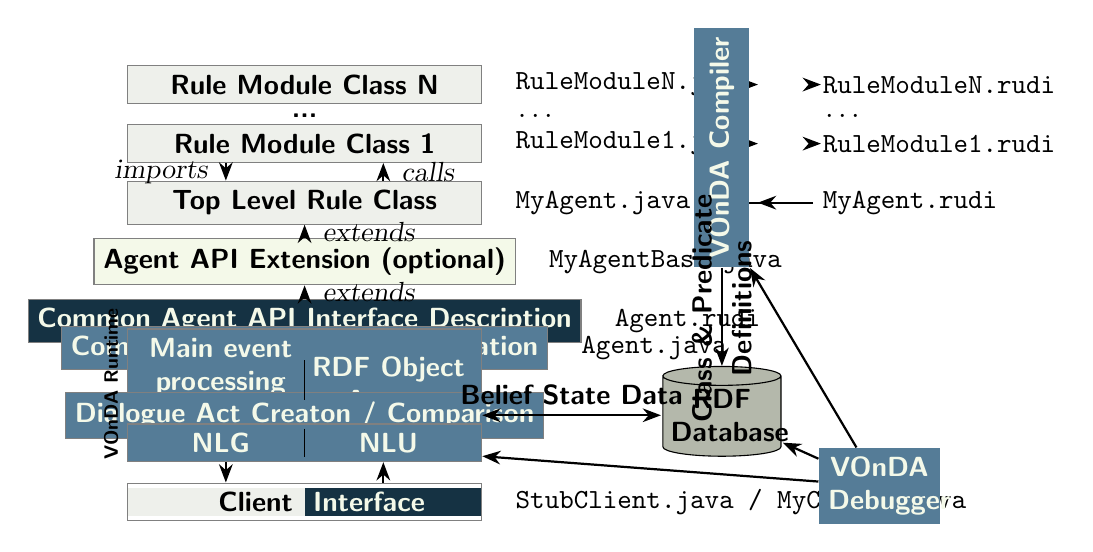
\begin{tikzpicture}[font=\bf\sffamily,
  box/.style={minimum width=4.5cm, minimum height=.35cm, draw=gray, text=black},
  gbox/.style={box, fill=lightgray},
  arr/.style={thick, -{Stealth}},
  larr/.style={thick, {Stealth}-},
  oarr/.style={thick, -{Stealth}},
  bbox/.style={box, fill=meddarkblue, text=ivory, draw},
  rbox/.style={node distance=0.3cm, font=\ttfamily},
  fbox/.style={node distance=4.2cm, font=\ttfamily},
  rlabel/.style={right, xshift=1mm, font=\sl},
  llabel/.style={left, xshift=-1mm, font=\sl}
]
\node[gbox](rmn) at (0,0.2) { Rule Module Class N };
\node[rbox, right= of rmn](rmnj){RuleModuleN.java};
\draw[larr] (rmnj) --  ++(1.5,0);
\node[fbox, right= of rmn](rmnr){RuleModuleN.rudi};
\draw[oarr] (rmnr) --  ++(-1.5,0);

\node[minimum width=4.5cm](ddd) at (0,-.2) { \normalsize ... };
\node[rbox, right= of ddd]{\small ...};
\node[fbox, right= of ddd]{\small ...};

\path (rmn) ++(0,-.75) node[gbox](rm1) { Rule Module Class 1 };
\node[rbox, right= of rm1](rm1j){RuleModule1.java};
\draw[larr] (rm1j) --  ++(1.5,0);
\node[fbox, right= of rm1](rm1r){RuleModule1.rudi};
\draw[oarr] (rm1r) --  ++(-1.5,0);

\path (rm1) ++(0,-.75) node[gbox](tlrc) { Top Level Rule Class };
\node[rbox, right= of tlrc](maj){MyAgent.java};
\draw[larr] (maj.east) ++(.35,0) --  ++(.72,0);
\node[fbox, right= of tlrc](mar){MyAgent.rudi};
\draw[oarr] (mar.west) -- ++(-.7,0);
\draw[arr] (tlrc.north) ++ (1,0) coordinate (tn) -- node[rlabel]{calls} (rm1.south -| tn);
\draw[arr] (rm1.south) ++ (-1,0) coordinate (rs) -- node[llabel]{imports} (tlrc.north -| rs);

\path (tlrc) ++(0,-.75) node[box, fill=ivory](caai)
  {Agent API Extension (optional)};
\node[rbox, right= of caai]{MyAgentBase.java};
\draw[arr] (caai) -- node[rlabel]{extends} (tlrc);

\path (caai) ++(0,-.75) node[box, fill=darkblue, text=ivory](caid) {Common Agent API Interface Description}
 ++ (0,-.35) node[bbox](caii) {Common Agent API Implementation}
% ++ (0,-.35) node[bbox] {VOnDA Runtime}
 ++ (0,-.45) node[bbox, minimum height=.6cm](cb) {
\begin{minipage}{2cm}\centering Main event\\processing loop\end{minipage}
\begin{minipage}{2cm}\centering RDF Object Access\end{minipage}
}
 ++ (0, -.4) node[bbox] {Dialogue Act Creaton / Comparison}
 ++ (0,-0.35) node[bbox](nlp){
\begin{minipage}{2cm}\centering NLG\end{minipage}
\begin{minipage}{2cm}\centering NLU\end{minipage}
};
\node[rotate=90,yshift=2mm] at (cb.west){\scriptsize VOnDA Runtime};

\node[rbox, right= of caii]{Agent.java};
\node[rbox, right= of caid]{Agent.rudi};
\draw[arr] (caid) -- node[rlabel]{extends} (caai);
\draw (cb) ++(0,.3) -- +(0,-.51);
\draw (nlp) ++(0,.18) -- +(0,-.36);

\path (nlp) ++(0,-.75)
+(-1.125,0) node[fill=lightgray, minimum width=2.25cm, minimum height=.35cm]{}
+(1.125,0) node[fill=darkblue, text=ivory, minimum width=2.25cm, minimum height=.35cm]{}
+(0,0) node[box](ci) {\hspace{2.7ex}Client\color{ivory}\ \ Interface };
\node[rbox, right= of ci]{StubClient.java / MyClient.java};

\draw[arr] (ci.north) ++ (1,0) coordinate (ci1) -- (nlp.south -| ci1);
\draw[arr] (nlp.south) ++ (-1,0) coordinate (nl1) -- (ci.north -| nl1);

\node[minimum width=2cm, minimum height=.7cm, %draw,
      fill=meddarkblue, text=ivory, rotate=90](vc) at (5.3,-.6) {\bf\sffamily VOnDA Compiler};

\node[minimum width=1.3cm, minimum height=.8cm, %draw,
      fill=meddarkblue, text=ivory](dbg) at (7.3,-4.9)
      {\begin{minipage}{1.3cm}\centering\bf\sffamily VOnDA\\Debugger\end{minipage}};

% SUPER TEMPLATE FÜR DIE "TONNE"
\path [fill=midgray, text=black, draw=black] (5.3, -4)
   node[minimum height=1.24cm,minimum width=1.5cm] (db) {\cmp{1.3cm}{RDF\\Database}}
   ++(-.75,0.5)
   -- ++(0,-.9)
   arc [start angle=180, delta angle=180, x radius=.75cm, y radius=1.2mm]
   -- ++(0,.9)
   arc[start angle=0, delta angle=360, x radius=.75cm, y radius=1.2mm];

\draw[arr] (vc) --
  node[above, rotate=90, xshift=1.1mm]{Class \& Predicate}
  node[below, rotate=90, xshift=1.1mm]{Definitions} (db);
\draw[arr, {Stealth}-{Stealth}] (db.west)
       -- node[above]{Belief State Data} (db.west -| cb.east);

\draw[arr](dbg) -- (nlp);
\draw[arr](dbg) -- (db);
\draw[arr](dbg) -- (vc.south west);
\end{tikzpicture}

%%% Local Variables:
%%% mode: latex
%%% TeX-master: "vonda"
%%% End:

  \caption{Schematic of a \vonda interaction manager implementation}
  \label{fig:architecture}
\end{figure}

A basic \vonda project consists of an ontology, a client interface to
connect the communication channels of the application to the agent,
and a set of rule files that are arranged in a tree, using
\texttt{include} statements. The blue core in
Figure~\ref{fig:architecture} is the run-time system that is part of
\vonda, while all light grey elements are the application specific
parts of the agent. A YAML project file contains all
necessary information for compilation: the ontology, the top-level
rule file and other parameters, like custom compile commands for
\vonda's debugger.

As you can see in the figure, instead of the top-level rule file
directly extending from the framework's abstract \texttt{Agent} class,
you can optionally insert a custom extension of this class and let the
rule agent derive from that. This is meant for special cases when the
Agent class functionality does not suffice or is not exactly the way
you need it (e.g., when more complex synchronisation is needed). Then,
you can use the configuration key \texttt{agentBase} with a fully
specified class name to extend the top-level generated file from your
custom agent base class.

The \vonda compiler translates rule files with the extension \texttt{.rudi} to
Java files. During this process, the ontology storing the RDF classes and
properties is used to automatically infer types, resolve whether field accesses
are actually accesses to the database, etc (see section
\ref{sec:typeinference}).
Every rule file can define variables and functions in \vonda syntax which are
then available to all included files.

The current structure assumes that most of the Java functionality that
is used inside the rule files will be provided by the \texttt{Agent}
superclass. There are, however, alternative ways to use other Java
classes directly (see section \ref{sec:javatypes} for further
info). You can either use Java helper classes and/or objects, which is
the preferred way, or you make the methods and fields from the custom
\texttt{agentBaseClass} available to all rule files. If the compiler
does not pick up the type definitions by itself, you can support it by
declaring fields and methods in the type definition file. In the
example of figure ~\ref{fig:architecture}, this would be
\texttt{MyAgent.rudi}).

\section{The \vonda Rule Language}
\label{sec:language}
\vonda's rule language looks very similar to Java/C++. There are a number of
specific features which make it much more convenient for the specification of
dialogue strategies. One of the most important features is the way objects in
the RDF store can be used throughout the code: RDF objects and classes can be
treated similarly to those of object oriented programming languages, including
the type inference and inheritance that comes with type hierarchies.

\subsection{The Structure of a \vonda File}

A \vonda file usually consists of a list of (possibly nested) rule statements,
often complemented by variable and function definitions. In this section, we
will describe the elements of the syntax in more detail.

\vonda does not require to group statements in some kind of high-level
structure like e.g. a class. It is, in fact, not possible to define classes in
\texttt{.rudi} files at all, rules and method declarations have to be put
directly into the rule file. The same holds for every kind of valid
(Java-) statement, like assignments, \texttt{for} loops etc. From this, the
compiler will create a Java class where the methods and rules that are
transformed are represented as methods of this specific (generated)
class. All other statements as well as auto-generated calls to the methods
representing the rules will be put into the \texttt{process()} method that
\vonda creates to build a rule evaluation cycle. In doing so, the execution
order of all statements, including the rules, is preserved.

This functionality offers possibilities to e.g. define and process high-level
variables that you might want to have access to in subsequent rules or to insert
termination conditions that prevent some rule executions.

\textbf{Warning:} Variables declared globally in a file will be
transformed to fields of the Java class. We found that in very rare
occasions, this can lead to unexpected behaviour when using them in a
propose or timeout block as well as changing them in a global
statement. As proposes and timeouts will not be exceuted immediately,
they need every variable used inside them to be effectively
final. \vonda leaves the evaluation of validness of variables for such
blocks to Java. We found that Java might mistakenly accept variables
that are not effectively final, which might lead to completely
unexpected behaviour when proposes and timeouts with changed variable
values are executed.

The only important exception, where globally defined variables and
methods persist throughout the whole runtime of the system are
variables defined in the top-level rule file. This is on purpose, and
can be used to define persistent variables also usable in lower-level
rule files, or to be accessed from other java code.

\subsection{Rules and rule labels}

The core of \vonda dialogue management are the dialogue rules, which will be
evaluated at run-time system on every trigger generated from the environment or
the internal processing.
A rule (optionally) starts with a name that is given as a Java-like label: an
identifier followed by a colon. Following this label is an
\texttt{if}-statement, with optional \texttt{else} case. The clause of the
\texttt{if}-statement expresses the condition under which the rule, or rather
the \texttt{if} block, is to be executed; in the \texttt{else} block you can
define what should happen if the condition is \texttt{false}, like stopping the
evaluation of (a sub-tree of) the rules if necessary information is missing.

\begin{figure}[htb]
\begin{small}
\begin{lstlisting}
intro:
  if (introduction) {
    is_user_known:
      if (user.unknown) {
        ask_for_name: if (talkative) askForName();
      } else {
        greetUser();
      }
  }
\end{lstlisting}
\end{small}\vspace{-2ex}
\caption{A simple rule}
\end{figure}

Rules can be nested to arbitrary depth, so \texttt{if}-statements inside a rule
body can also be labelled. The labels are a valuable tool for debugging the
system at run-time, as they can be logged live with the debugger GUI
(cf. chapter \ref{sec:debugger}). The debugger can show you which rules were
executed when and what the individual results of each base clause of the
conditions were.

\subsection{The \texttt{propose} and \texttt{timeout} constructs}

There are two statements with a special syntax and semantics: \texttt{propose}
and \texttt{timeout}. \texttt{propose} is \vonda's current way of implementing
probabilistic selection. All (unique) propose blocks that are in active rule
actions are collected, frozen in the execution state in which they were
encountered, like closures known from functional programming languages. When
all possible proposals have been selected, a statistical component decides
on the ``best'', whose closure is then executed.

\begin{figure}[h]
  \centering\small%
\begin{lstlisting}
if (!saidInSession(#Salutation(Meeting)) {
  // Wait 7 secs before taking initiative
  timeout("wait_for_greeting", 7000) {
    if (! receivedInSession(#Greeting(Meeting))
      propose("greet") {
        da = #InitialGreeting(Meeting);
        if (user.name) da.name = user.name;
        emitDA(da);
      }
  }

  if (receivedInSession(#Salutation(Meeting))
    propose("greet_back") { // We assume we know the name by now
      emitDA(#ReturnGreeting(Meeting, name={user.name});
    }
  }
}
\end{lstlisting}\vspace*{-3ex}
  \caption{\label{fig:propose}\texttt{propose} and \texttt{timeout} code example}
\end{figure}

\texttt{timeout}s generate the same kind of closures, but with a different
purpose. They can for example be used to trigger proactive behaviour, or to
check the state of the system after some amount of time, or in regular
intervals. A timeout will only be created if there is no active timeout with
the same name, otherwise, if the time delay is different than that of the last
\texttt{timeout} call, the delay will be set to the new value. For special
needs, the functions in figure~\ref{tbl:timeoutfns} are useful to achieve
specific behaviours based on \texttt{timeout}s.

\begin{figure}[htb]
\begin{tabular}{lp{.65\textwidth}}
\texttt{isTimedOut(\emph{label})}& returns \texttt{true} if a timeout with that
  label fired. This can be reset only by calling
  \texttt{removeTimeout(\emph{label})}, and is especially convenient to
  implement timeouts that should only be triggered once in a session. \\
\texttt{removeTimeout(\emph{label})}& see \texttt{isTimedOut(\emph{label})}\\
\texttt{cancelTimeout(\emph{label})}& cancels an \emph{active} timeout if there
                                      is one, has no effect otherwise \\
\texttt{hasActiveTimeout(\emph{label})}& returns true if there is an
  active timeout with that label \\
\end{tabular}
\caption{\label{tbl:timeoutfns}Functions for fine tuning \texttt{timeout} behaviour}
\end{figure}

There are two variants of \texttt{timeout}: \emph{labeled timeouts}, like the
one in the previous example which run out after the specified time (unless they
are cancelled before running out) and then execute their body, and
\emph{behaviour timeouts}, where the first argument is a dialogue act (see next
section) instead of a label. These are executed either when the specified time
is up or the behaviour that was triggered by the dialogue act is finished
(e.g. the audio generated by a text-to-speech engine ended, or a specified
motion came to an end), whatever comes first.

The following code patterns may help to use the different possibilities that
timeouts offer:

{\small%
\begin{lstlisting}
// timeout triggered exactly once per session
if (! hasActiveTimeout("robot_starts") && ! isTimedOut("robot_starts"))
  timeout("robot_starts", 4000) { ... }

// timeout reoccurring every 1000 milliseconds
if (! hasActiveTimeout("reptimeout"))
  timeout("reptimeout", 1000) { ... }

// ensure that something happens even if the expected condition does not
// become true after 10 seconds
if (! condition && ! hasActiveTimeout("ensure_cond")) {
  timeout("ensure_cond", 10000) {
    if (! condition) {
      // clean up
    }
  }
}
\end{lstlisting}}

\subsection{Stopping Rule Evaluation}
\label{sec:cancelrules}
There are multiple ways to stop rule evaluation locally (i.e. skipping the
evaluation of the current subtree) or globally (i.e. stopping the whole
evaluation cycle).
You can skip the evaluation of a specific rule you are currently in with the
statement \texttt{break label\_name;}. This will only stop the rule with the
respective label (no matter how deep the break statement is nested in it), such
that the next following rule is evaluated next.

If the evaluation is cancelled with the keyword \texttt{cancel}, all of the
following rules in the current file will be skipped (including any included
rule files). If the keyword \texttt{cancel\_all} is used, none of the following
rules, neither local nor higher in the rule tree, will be evaluated. This is
the \vonda way of deciding to not further evaluate whatever triggered the
current evaluation cycle and will mostly be used as an 'emergency exit', as the
dialogue rules should be rejecting any non-matching trigger by themselves.

To leave \texttt{propose} and \texttt{timeout} blocks, you need to use a
\texttt{return} statement without return value, as they are only reduced
representations of normal function bodies.

A detailed description of how the rules of a \vonda project are evaluated will
follow in section~\ref{sec:ruleevaluation}.


\subsection{RDF access and functional vs. relational properties}
\label{sec:rdfaccesses}

\begin{figure}[htb]
\rule{7mm}{0pt}\begin{minipage}{0.45\columnwidth}
\small%
\begin{lstlisting}[numbers=left,numberstyle=\scriptsize]
user = new Animate;
user.name = "Joe";
set_age:
if (user.age <= 0) {
  user.age = 15;
}
\end{lstlisting}
\end{minipage}\vrule\hspace{1ex}
\begin{minipage}{0.44\columnwidth}
    \small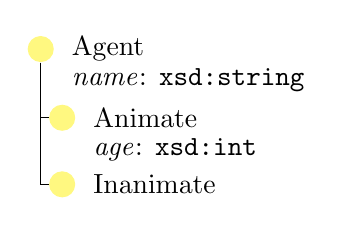
\begin{tikzpicture}[
  blob/.style={circle, fill=yellow!50!white, minimum width=2mm},
  txt/.style={node distance=3mm}]
  \draw (0,0) node (agent) [blob]{};
  % BEWARE: RIGHT OF= IS DEPRECATED, DON'T USE IT
  \node (agtxt) [right= 0.1 of agent, txt] {Agent};
  \node (name) [below= 0.4 of agtxt.west, anchor=west]{\emph{name}: \texttt{xsd:string}};
  \node (animate) [blob, below=0.7 of agtxt.west]{};
  \node (antxt) [right= 0.1 of animate, txt] {Animate};
  \node (name) [below= 0.4 of antxt.west, anchor=west]{\emph{age}: \texttt{xsd:int}};
  \node (inanimate) [blob, below= 0.5 of animate, node distance=9mm]{};
  \node (intxt) [right= 0.1 of inanimate, txt] {Inanimate};
  \draw (agent) |- (animate);
  \draw (agent) |- (inanimate);
\end{tikzpicture}
\end{minipage}
  \caption{Ontology and \vonda code}
  \label{fig:rdfobjects}
\end{figure}

Figure \ref{fig:rdfobjects} shows an example of \vonda code, and how it relates
to RDF type and property specifications, schematically presented on the right.
The domain and range definitions of properties are picked up by the compiler
and then used in various places, e.g., to infer types, do automatic code or
data conversions, or create ``intelligent'' boolean tests, like in line 4,
which will expand into two tests, one testing for the existence of the property
for the object, and in case that succeeds, a test if the value is smaller or
equal than zero.

The connection of \vonda to the ontology loaded into HFC during compile time
enables the compiler to recognise the correct RDF class to create a new
instance when creating a new RDF object with \texttt{new}, similar to a Java
object, and to resolve field/property accesses to all RDF instances. Field
accesses as shown in line 2 and 3 of figure \ref{fig:property-access} will be
analysed and transformed into database accesses. Object creation or
assignments, i.e. changes to existing objects, will be immediately reflected in
the database.


\begin{figure}[htbp]
\small\begin{minipage}{0.5\textwidth}
\begin{lstlisting}[numbers=left,numberstyle=\scriptsize]
c = new Child;
nm = c.name;
c.name = "new name";
Set middle = c.middleNames;
c.middleNames += "John";
c.middleNames -= "James";
c.middleNames = null;
\end{lstlisting}
\end{minipage}{\LARGE$\Rightarrow$}\rule{6.4cm}{0pt}\\
\begin{minipage}{0.99\textwidth}
\begin{lstlisting}[numbers=left,numberstyle=\scriptsize]
c = palAgent._proxy.getClass("<dom:Child>").getNewInstance(palAgent.DEFNS);
nm = c.getString("<upper:name>");
c.setValue("<upper:name>", "new name");
middle = c.getValue("<upper:middleNames");
c.getValue("<upper:middleNames>").add("John");
c.getValue("<upper:middleNames>").remove("James");
c.clearValue("<upper:middleNames>");
\end{lstlisting}
\end{minipage}
  \caption{Examples for an RDF property access}
  \label{fig:property-access}
\end{figure}

\vonda will also draw type information from the database. If the name property
of the RDF class \texttt{Child} is of type \texttt{String}, exchanging line 2
by the line \texttt{int name = c.name} will result in a warning of the
compiler. During this process, the compiler will automatically also use the
correspondence of XSD and Java types shown in figure \ref{fig:RdfToJava}.

\begin{figure}[htb]
{\small\ttfamily\begin{center}
\begin{tabular}{ll@{\hspace{8em}}ll}
<xsd:int> & Integer & <xsd:integer> & Long\\
<xsd:string> & String & <xsd:byte> & Byte\\
<xsd:boolean> & Boolean & <xsd:short> & Short\\
<xsd:double> & Double & <xsd:dateTime> & Date\\
<xsd:float> & Float & <xsd:date> & XsdDate\\
<xsd:long> & Long & <xsd:dateTimeStamp> & Long
\end{tabular}\end{center}}\vspace{-2ex}
\caption{\label{fig:RdfToJava}Standard RDF types and the Java types as which they will be recognized}
\end{figure}

If there is a chain of more than one field/property access, every part is
tested for existence in the target code, keeping the source code as concise as
possible (see also figure~\ref{tab:multi-predaccess} in
section~\ref{sec:typeinference}). Also for reasons of brevity, the type of a
new variable needs not be given if it can be inferred from the value assigned
to it.

Moreover, \vonda determines whether an access is made using functional or
relational predicates and will handle it accordingly, assuming a collection
type if necessary. In the rule language, the operators \texttt{+=} and
\texttt{-=} are overloaded. They can be used with sets and lists as shortcuts
for adding and deleting objects. \texttt{a += b} will be compiled to
\texttt{a.add(b)} and \texttt{a -= b} results in \texttt{a.remove(b)}, as shown
in figure~\ref{fig:property-access}.

\paragraph{Creating RDF instances with
  \texttt{new}}\label{sec:new_rdf}

In figure~\ref{fig:property-access}, \texttt{c = new Child;} is used
to create a new RDF instance of class \texttt{Child}. Since every RDF
instance must be part of a namespace, a default namespace string
variable \texttt{DEFNS} is defined in the \texttt{Agent} class. Its
default value is \texttt{"def"}, which corresponds to the long URI
\texttt{http://www.dfki.de/lt/default.owl\#}. You can change this
variable to any value in the initialisation code of your agent (it
should be a valid short namespace name)\footnote{see also the
  \texttt{init} method of \texttt{ChatAgent} from the example project},
and all RDF objects created in the generated \vonda code will then be
created in your custom namespace.

\paragraph{Parameterising field access}\label{sec:field_access_expansion}

To be able to \emph{parameterise} the field access to RDF objects,
\vonda has a special mechanism. Instead of the above
\texttt{c.middleNames}, you could have done the following:

\begin{lstlisting}
mid = "<upper:middleNames>";
Set middle = c.{mid};
\end{lstlisting}

if you use \verb|{<exp>}| in a field access, the compiler assumes
\texttt{exp} to evaluate to a \texttt{String}, and the string
resulting from evaluating \texttt{exp} at runtime will be used as if
you would have specified an identifier with the same name. Be aware
that this only works for access to RDF objects, and that you have to
take care of all type checking and casting by yourself, since the
compiler can not figure out in advance which properties you will access.

\subsection{Casting types in \vonda}
\label{sec:cast}

The syntax for casting expressions explicitely to a specific type is
slightly different than the Java syntax, for reasons of better
readability and easier treatment in parsing the code. \vonda uses the
\texttt{isa} keyword as infix operator, similar to the \texttt{cast()}
in C++, so a Java-style cast \texttt{((Child)c)} will be
\texttt{isa(Child, c)} in \vonda syntax

\subsection{Type inference and overloaded operators}
\label{sec:typeinference}

\vonda allows static type assignments and casting, but in many cases these can
be avoided. If, for example, the type of the expression on the right-hand side
of a declaration assignment is known or inferrable, it is not necessary to
explicitely state it.

You can also declare variables final.

\begin{figure}[htbp]
  \begin{small}
\begin{minipage}{.55\textwidth}
\begin{lstlisting}
if (! c.user.personality.nonchalance){ ... }
\end{lstlisting}
\end{minipage}\rule{2cm}{0pt}{\LARGE$\Rightarrow$}\hfill\\
\begin{lstlisting}
if (!((((c != null) && (c.user != null)) && (c.user.personality != null))
      && (c.user.personality.nonchalance != null))) {
  ...
}
\end{lstlisting}\end{small}\vspace*{-2ex}
\caption{\label{tab:multi-predaccess}Transformation of complex boolean expressions}

\end{figure}
\vspace*{10pt}

A time-saving feature of \vonda which also improves readability is the
automatic completion of boolean expressions in the clauses of \texttt{if},
\texttt{while} and \texttt{for} statements. As it is obvious in these cases
that the result of the expression must be of type boolean. \vonda automatically
fills in a test for existence if it is not. When encountering field accesses,
it makes sure that every partial access is tested for existence (i.e., not
\texttt{null}) to avoid a \texttt{NullPointerException} in the runtime
execution of the generated code.

Be aware that the expansion in the figure only occurs if the multiple field
access is used as boolean test. In the following example, the first clause in
the boolean expression should not be omitted, since a
\texttt{NullPointerException} could still occur because the second clause does
not trigger an automatic test for existence of the \texttt{status} of
\texttt{activity}:

\begin{lstlisting}
if (activity.status && activity.status == "foo"){ ... }
\end{lstlisting}

Many operators are overloaded, especially boolean operators such as
\textbf{\texttt{<=}}, which compares numeric values, but can also be used to
test if an object is of a specific class, for subclass tests between two
classes, and for subsumption of dialogue acts.

\begin{figure}[htbp]
\centering
{\footnotesize%
\begin{minipage}{0.28\textwidth}
\begin{lstlisting}
if (sa <= #Question){
  ...
}
\end{lstlisting}
\end{minipage}\vline\hspace{1em}
\begin{minipage}{0.6\textwidth}
\begin{lstlisting}
if (sa.isSubsumedBy(new DialogueAct("Question")) {
  ...
}
\end{lstlisting}
\end{minipage}}\vspace*{-2ex}
\caption{\label{tab:overloaded-comparison}Overloaded comparison operators}
\end{figure}

\subsection{Dialogue Acts}
\label{sec:caret}

A central functionality of a dialogue system is receiving and emitting dialogue
acts that result from a user utterance resp. can be transformed to natural
language by a generation component to communicate with the user. In \vonda,
the function for sending dialogue acts is called \texttt{emitDA}.

The dialogue act representation is an internal feature of \vonda. We are
currently using the DIT++ dialogue act hierarchy \citep{bunt2012iso} and
shallow frame semantics along the lines of FrameNet
\citep{ruppenhofer2016framenet} to represent dialogue acts. The natural
language understanding and generation units connected to \vonda should
therefore be able to generate or, respectively, process this representation.

\begin{figure}[htb]
  \centering\small\texttt{emitDA(\#Inform(Answer, what=\{solution\}));}
  \vspace*{-1ex}\caption{\label{fig:DA}Dialogue Act Example}
\end{figure}

Figure \ref{fig:DA} shows the dialogue act representation in \vonda, as passed
to, e.g., the \texttt{emitDA} function. \texttt{Inform}\verb|(...)| will be
recognized by \vonda as dialogue act because it has been marked with
\verb|#|. It will then create a new instance of the class DialogueAct that
contains the respective modifications. As a default, arguments of a DialogueAct
creation (i.e., character strings on the left and right of the equal sign) are
seen as and transformed to constant (string) literals, because most of the time
that is what is needed.  Surrounding a character sequence with curly brackets
(\texttt{\{\}}) marks it as an expression that should be evaluated. In fact,
arbitrary expressions are allowed inside the curly brackets, and converted
automatically to a string, if necessary and possible.

While this kind of shallow semantics is enough for many applications, we
already experience its shortcomings when trying to handle, for example, social
talk. One of the next improvements will be the extension of Dialogue Acts to
allow for embedded structures.


\subsection{Declaring External Methods And Fields}
\label{sec:javatypes}

As mentioned before, you can use every method or field you declare in
some Java class or your custom \texttt{Agent} subclass implementation
in your \vonda code. Their declaration in the Java/rudi interface
looks like a normal Java field or method definition
(cfg. figure~\ref{tab:javadef}). It is possible to use generics in
these definitions, although their names are, for complexity reasons,
restricted to one single uppercase letter.

\begin{figure}[htbp]
\small
\begin{lstlisting}
MyType someVariable;          // field of class MyType
MyType someFun(ClA a, ClB b); // method someFun with signature
                              // (ClA, ClB) --> MyType
                              // return type can be void for a procedural method
\end{lstlisting}\vspace*{-2ex}
\caption{\label{tab:javadef}Defintions of existing Java fields and methods for
  \vonda}
\end{figure}

There is a variety of standard Java methods called on Java classes that \vonda
automatically recognises, like e.g. the \texttt{substring} method for
Strings. If you find that you need \vonda to know the signature of a new method
or a field that is defined in some other class that is not your \texttt{Agent}
subclass, you can provide \vonda with knowledge about them by adding their
definition to the interface as follows:

\begin{figure}[htbp]
\centering
\small
\begin{lstlisting}
#SomeClass myType Function(typeA a); // declaration of SomeClass method
#SomeClass myType someVar;           // declaration of SomeClass field
#List<T> T get(int a);               // use of Generics is possible and
                                     // used in type inference
\end{lstlisting}\vspace*{-2ex}
\caption{\label{tab:methoddef}Definition of a non-static method of Java objects}
\end{figure}

It is important to realise that all declarations in the interface are only
compile time information for \vonda and will not be transferred to the compiled
code, whereas declarations in the rule code itself will also appear in the
compiled code.

\subsubsection{Functional constructs}

\vonda allows to specify \texttt{Function} arguments, where lambda
constructions can then be used in the code. Currently, the functions listed in
figure \ref{tab:lambda-functions} are pre-defined in the \texttt{Agent} class.
If you for example want to filter a set of RDF objects by a sub-type relation,
you can write:
{\small\begin{lstlisting}
des = filter(agent.desires, lambda(d) (d <= UrgentDesire));
\end{lstlisting}}
or
{\small\begin{lstlisting}
des = filter(agent.desires, lambda(d) { return (d <= UrgentDesire); });
\end{lstlisting}}

\begin{figure}[htbp]
\small%
\begin{lstlisting}
boolean some(Collection<T> coll, Function<Boolean, T> pred);
boolean all(Collection<T> coll, Function<Boolean, T> pred);
List<T> filter(Collection<T> coll, Function<Boolean, T> pred);
List<T> sort(Collection<T> coll, Function<Integer, T, T> comp);
Collection<T> map(Collection<S> coll, Function<T, S> f);
int count(Collection<T> coll, Function<Boolean, T> pred);
T first(Collection<T> coll, Function<Boolean, T> pred);
\end{lstlisting}\vspace*{-2ex}
\caption{\label{tab:lambda-functions}Functions that take lambda expressions as an argument}
\end{figure}


\subsubsection{Using rules of other rule files with \texttt{include}}

With the \texttt{include} statement, e.g. \texttt{include RuleFile;},
which needs to appear at the root level of rule files, the (compiled)
rules and definitions in \texttt{RuleFile.rudi} and its included files
are added at the position of the \texttt{include}. This is not a
macro-like inclusion, the compiler generates Java classes for every
\texttt{include}.

This inclusion has two important effects. On the one hand, it triggers
the compilation of the included file at exactly this point, such that
any fields and methods known at this time will be available in the
included file. On the other hand, all the rules contained in the
included file will be inserted in the run-time rule cycle at the
specific position of the \texttt{include}, that is, in the resulting
code the \texttt{process()} method of the generated code for the
included file will be executed.

\texttt{include} makes it possible to organize the rules and local
declarations of a project into meaningful sub-units. This supports
modularity, as different subtrees of the \texttt{include} hierarchy can
easily be added, moved, taken away or re-used in different projects.

\subsubsection{Java-Code verbatim in rule files} \label{sec:rudi-verbatim}

To maintain simplicity, \vonda intentionally only provides limited Java
functionalities. Whatever is not feasible in \vonda source code should be done
in methods in the wrapper class or other helper classes.

In cases where this is not possible and you urgently need a
functionality of Java that \vonda cannot parse or represent correctly,
you can use the verbatim inclusion feature. Everything between
\verb|/*@| and \verb|@*/| will be treated like a multi-line Java
comment, meaning the content is not parsed or evaluated further. It
will be transferred to the compiled code as is into the intended
position.

It is strongly discouraged to use this feature extensively, but to use
helper objects/classes instead whereever possible. Not only will code
written this way likely become unreadable if there is too much of it,
it might also not be portable to new \vonda versions, if the way of
generating the Java code changes.

\subsubsection{Java \texttt{import}
  statements} \label{sec:java-import}

You can use \texttt{import} statements as in Java syntax in rule
files, but only at the very beginning. You should however be aware
that \vonda will not know that these classes have been imported, nor
their methods and fields. It will however accept creations of
instances of unknown classes, as well as your casting of results of
unknown methods. If you want \vonda to have type information about
methods called on instances on one of these classes, you can put this
information into your \texttt{typeDef} file (see the beginning of this
section).

\section{The Run-Time System}

The run-time library contains the basic functionality for handling the rule
processing, including the proposals and timeouts, and for the on-line
inspection of the rule evaluation. There is, however, no blueprint for the main
event loop, since that depends heavily on the host application. The run-time
library also contains methods for the creation and modification of shallow
semantic structures (\texttt{DialogueAct}s), and especially for searching the
interaction history for specific utterances. Most of this functionality is
available through the abstract \texttt{Agent} class, which needs to be extended
to a concrete subclass for your application.

There is also functionality to talk directly to the HFC database using queries
(see section \ref{sec:hfc_usage}), in case the object view that was
described in before is not sufficient or too awkward.

\subsection{Rule Evaluation Cycle}
\label{sec:ruleevaluation}

Your \vonda rule files form a tree, starting at the top-level file that you
specify in the configuration file, and the \texttt{include}d rule files. The
evaluation of the rule starts in the top-level files and proceeds in pre-order
through this tree. If you use a \texttt{cancel} or \texttt{cancel\_all}
statement (cf. section~\ref{sec:cancelrules}), the rule evaluation will be
either locally or globally stopped.

The set of your reactive \vonda rules is executed whenever there is a change in
the information state, which is stored in the database. These changes can be
caused by incoming sensor or application data, intents from the speech
recognition, or expired \texttt{timeout}s.  A rule can have direct effects,
like changes in the information state, or system calls. Furthermore, the
\texttt{proposal}s, which are (labeled) blocks of code in a frozen state that
will not be immediately executed, but collected, similar to closures.

All rules are repeatedly applied until a fix point is reached: No new proposals
are generated and there is no change of the information state in the last
iteration. Then, the set of collected proposals is evaluated by a statistical
component, which will select the best alternative. This component can be
exchanged to make it as simple or elaborate as necessary, which also allows to
take into account arbitrary features from the data storage.

At the start of your program, an object of the generated top-level
class will be created which will exist as long as the program is
executed. For the execution of embedded rules, temporary objects will
be created, which cease to exist as soon as all relevant rules of the
subtree have been evaluated. As a consequence, no values created in
these objects will survive the rule evaluation if they are not stored
in a persistent location (e.g., a top-level variable or the database).

The embedded rules have access to all the variables and methods
declared in higher-level rule files, and all the values produced up to
their call (see also \ref{sec:volatile})

\subsection{Functionality Provided by the Run-Time System}
The following methods are declared in \texttt{src/main/resources/Agent.rudi};
their implementation is provided by Java itself or the \vonda framework.

\vspace*{2ex}

\newcommand{\pgr}[1]{\noindent\textbf{#1}}

\pgr{Pre-added Java methods}
\begin{small}
\begin{lstlisting}
#Object boolean equals(Object e);
#String boolean startsWith(String s);
#String boolean endsWith(String s);
#String String substring(int i);
#String String substring(int begin, int end);
#String boolean isEmpty();
#String int length();

#List<T> T get(int a);
#Collection<T> void add(Object a);
#Collection<T> boolean contains(Object a);
#Collection<T> int size();
#Collection<T> boolean isEmpty();
#Map<S, T> boolean containsKey(S a);
#Map<S, T> T get(S a);
#Array<T> int length;
\end{lstlisting}
\end{small}

\pgr{Short-hand conversion methods from Agent}
\begin{small}
\begin{lstlisting}
int toInt(String s);
float toFloat(String s);
double toDouble(String s);
boolean toBool(String s);
String toStr(T i);  // T in (int, short, byte, float, double, boolean)
\end{lstlisting}
\end{small}

\pgr{Other Agent methods}
\begin{small}
\begin{lstlisting}
// Telling the Agent that something changed
void newData();

String getLanguage();

// Random methods
int random(int limit); // return and int between zero and limit (excluded)
float random();        // return a random float between zero and one (excluded)
T random(Collection<T> coll); // select a random element from the collection

long now();     // return the current time since the epoch in milliseconds

Logger logger;  // Global logger instance

// discarding actions and shutdown
void clearBehavioursAndProposals();
void shutdown();
\end{lstlisting}
\end{small}

\pgr{Timeouts}
\begin{small}
\begin{lstlisting}
void newTimeout(String name, int millis);
boolean isTimedOut(String name);
void removeTimeout(String name);
boolean hasActiveTimeout(String name);
// cancel and remove an active timeout, will not be executed
void cancelTimeout(String name);
\end{lstlisting}
\end{small}

\pgr{Methods dealing with dialogue acts}
\begin{small}
\begin{lstlisting}
// sending of dialogue acts
DialogueAct createEmitDA(DialogueAct da);
DialogueAct emitDA(int delay, DialogueAct da);
DialogueAct emitDA(DialogueAct da);
#DialogueAct String getDialogueActType();
#DialogueAct void setDialogueActType(String dat);
#DialogueAct String getProposition();
#DialogueAct void setProposition(String prop);
#DialogueAct boolean hasSlot(String key);
#DialogueAct String getValue(String key);
#DialogueAct void setValue(String key, String val);
#DialogueAct long getTimeStamp();

// Access to dialogue acts of the current session
// my last outgoing resp. the last incoming dialogue act
DialogueAct myLastDA();
DialogueAct lastDA();

// Did I say something like ta in this session (subsumption)? If so, how many
// utterances back was it? (otherwise, -1 is returned)
int saidInSession(DialogueAct da);
// like saidInSession, only for incoming dialogue acts
int receivedInSession(DialogueAct da);

// Check if we asked a question that is still pending
boolean waitingForResponse();
// Mark last incoming DA as treated and not pending anymore (stop rules firing)
void lastDAprocessed();

DialogueAct addLastDA(DialogueAct newDA);
#DialogueAct void setProposition(String prop);
\end{lstlisting}
\end{small}

\pgr{Functions allowing lambda expressions (functional arguments)}
\begin{small}
\begin{lstlisting}
boolean some(Collection<T> coll, Function<Boolean, T> pred);
boolean all(Collection<T> coll, Function<Boolean, T> pred);
List<T> filter(Collection<T> coll, Function<Boolean, T> pred);
List<T> sort(Collection<T> coll, Function<Integer, T, T> c);
Collection<T> map(Collection<S> coll, Function<T, S> f);
int count(Collection<T> coll, Function<Boolean, T> pred);
T first(Collection<T> coll, Function<Boolean, T> pred);
\end{lstlisting}
\end{small}

\pgr{Methods on \texttt{Rdf} and \texttt{RdfClass} objects}
\begin{small}
\begin{lstlisting}
Rdf toRdf(String uri);
#Rdf String getURI();
#Rdf boolean has(String predicate);
#Rdf long getLastChange(boolean asSubject, boolean asObject);

RdfClass getRdfClass(String s);
boolean exists(Object o);

// return only the name part of an URI (no namespace or angle brackets)
String getUriName(String uri);
\end{lstlisting}
\end{small}


%%% Local Variables:
%%% mode: latex
%%% TeX-master: "userguide"
%%% End:

%\newpage
\section{Debugger/GUI}
\label{sec:debugger}

\vonda comes with a GUI \citep{rudibuggerThesis} that helps navigating, compiling and editing the source files belonging to a project. It can also be attached to your \vonda project at runtime to support debugging by logging the evaluation of rule conditions.

\begin{figure}[thb]

  \centering
  \includegraphics[width=.8\textwidth]{VondaGui.png}
  \caption{The \vonda GUI window}
  \label{vondagui}
\end{figure}

For further details, please take a look into rudibuggers own documentation. The project can be found on \url{https://github.com/yoshegg/rudibugger}.
\newpage
\section{The RDF Database HFC} \label{sec:hfc}

\vonda follows the information state/update paradigm. The information state is
realized by an RDF store and reasoner with special capabilities
(HFC \cite{krieger2013efficient}), namely the
possibility to directly use $n$-tuples instead of triples. This allows to
attach temporal information to every data chunk \cite{Krieger:FOIS2012,
  krieger2014detailed}. In this way, the RDF store can represent \emph{dynamic
  objects}, using either \emph{transaction time} or \emph{valid time}
attachments, and as a side effect obtain a complete history of all changes.
HFC is very efficient in terms of processing speed and memory footprint, and
has also provides some stream reasoning facilities. \vonda can use HFC
either directly as a library or as a remote server.
% , also allowing for more than one instance if needed (for this
% feature see section \ref{sec:2ndHfc}).

The following is the syntax of HFC queries (EBNF):
\begin{table}[htbp]
  \centering\small
\begin{verbatim}
<query>     ::= <select> <where> [<filter>] [<aggregate>] | ASK <groundtuple>
<select>    ::= {"SELECT" | "SELECTALL"} ["DISTINCT"] {"*" | <var>^+}
<var>       ::= "?"{a-zA-Z0-9}^+ | "?_"
<nwchar>    ::= any NON-whitespace character
<where>     ::= "WHERE" <tuple> {"&" <tuple>}^*
<tuple>     ::= <literal>^+
<gtuple>    ::= <constant>^+
<literal>   ::= <var> | <constant>
<constant>  ::= <uri> | <atom>
<uri>       ::= "<" <nwchar>^+ ">"
<atom>      ::= "\""  <char>^* "\"" [ "@" <langtag> | "^^" <xsdtype> ]
<char>      ::= any character, incl. whitespaces, numbers, even '\"'
<langtag>   ::= "de" | "en" | ...
<xsdtype>   ::= "<xsd:int>" | "<xsd:long>" | "<xsd:float>" | "<xsd:double>" |
                "<xsd:dateTime>" | "<xsd:string>" | "<xsd:boolean>" | "<xsd:date>" |
                "<xsd:gYear>" | "<xsd:gMonthDay>" | "<xsd:gDay>" | "<xsd:gMonth>" |
                "<xsd:gYearMonth>" | "<xsd:duration>" | "<xsd:anyURI>" | ...
<filter>    ::= "FILTER" <constr> {"&" <constr>}^*
<constr>    ::= <ineq> | <predcall>
<ineq>      ::= <var> "!=" <literal>
<predcall>  ::= <predicate> <literal>^*
<predicate> ::= <nwchar>^+
<aggregate> ::= "AGGREGATE" <funcall> {"&" <funcall>}^*
<funcall>   ::= <var>^+ "=" <function> <literal>^*
<function>  ::= <nwchar>^+
\end{verbatim}
  \caption{BNF of the database query language}
  \label{tab:hfcquerybnf}
\end{table}

%\paragraph{Notes}

The reserved symbols \texttt{ASK}, \texttt{SELECT}, \texttt{SELECTALL},
\texttt{DISTINCT}, \texttt{WHERE}, \texttt{FILTER} and \texttt{AGGREGATE}
do \emph{not} need to be written in uppercase, but neither \texttt{filter} predicates nor \texttt{aggregate} functions should be named like reserved symbols.

\emph{don't-care} variables should be marked \emph{explicitely} by using
\verb|?_|, particularly if \texttt{SELECT} is used with \verb|*| as in:
\begin{verbatim}
     SELECT DISTINCT * WHERE ?s <rdf:type> ?_
     SELECT * WHERE ?s <rdf:type> ?o ?_
\end{verbatim}
To put a restriction on the object position you can also use
\emph{don't-care} variables and filters:

\begin{verbatim}
     SELECT ?s WHERE ?s <rdf:type> ?o ?_ FILTER ?o != <foo-class>
\end{verbatim}

Aggregates in HFC take whole tables or parts of them and calculate a result based on their entities. As the type of aggregates and filter functions cannot be overloaded, there are multiple similar functions for different types, e.g. F for \texttt{float}, L for \texttt{long}, D for \texttt{double}, I
for \texttt{int}, and S for \texttt{String}.

\begin{table}[htbp]
  \centering
 \begin{tabular}{lll}
   CountDistinct&  FSum&             LMax\\
   Count&          FMean&            LMean\\
   DMean&          LGetFirst2&       LMin\\
   DSum&           LGetLatest2&      LSum\\
   DTMax&          LGetLatest&       LGetLatestValues\\
   DTMin&          LGetTimestamped2& Identity     \\
 \end{tabular}
  \caption{Available aggregates}
  \label{tab:hfcaggregates}
\end{table}

Apart from \verb|==| and \verb|!=|, functional operators can be used in \texttt{filter} expressions as well. As for aggregates, there are multiple versions of the same function for different data types.

\begin{table}[htbp]
  \centering\small
\begin{tabular}{llll}
CardinalityNotEqual &        FNotEqual &               IntStringToBoolean &      LMin \\
Concatenate &                FProduct &                IProduct &                LNotEqual \\
DTIntersectionNotEmpty &     FQuotient &               IQuotient &               LProduct \\
DTLessEqual &                FSum &                    IsAtom &                  LQuotient \\
DTLess &                     GetDateTime &             IsBlankNode &             LSum \\
DTMax2 &                     GetLongTime &             IsNotSubtypeOf &          LValidInBetween\\
DTMin2 &                     HasLanguageTag &          ISum &                    MakeBlankNode \\
EquivalentClassAction &      IDecrement &              IsUri &                   MakeUri \\
EquivalentClassTest &        IDifference &             LDecrement &              NoSubClassOf \\
EquivalentPropertyAction &   IEqual &                  LDifference &             NoValue \\
EquivalentPropertyTest &     IGreaterEqual &           LEqual &                  PrintContent \\
FDecrement &                 IGreater &                LGreaterEqual &           PrintFalse \\
FDifference &                IIncrement &              LGreater &                PrintSize \\
FEqual &                     IIntersectionNotEmpty &   LIncrement &              PrintTrue \\
FGreaterEqual &              ILessEqual &              LIntersectionNotEmpty &   SameAsAction \\
FGreater &                   ILess &                   LIsValid &                SameAsTest \\
FIncrement &                 IMax2 &                   LLessEqual &              SContains.java\\
FLessEqual &                 IMax &                    LLess &                   UDTLess \\
FLess &                      IMin2 &                   LMax2 \\
FMax &                       IMin &                    LMax \\
FMin &                       INotEqual &               LMin2 \\
\end{tabular}
\caption{Available filter functions}
  \label{tab:hfcfunctions}
\end{table}

\subsection{Usage of HFC in \vonda} \label{sec:hfc_usage}

The RDF store contains the dynamic and the terminological knowledge:
specifications for the data objects and their properties, as well as a
hierarchy of  dialogue acts,  semantic frames and their arguments. These
specifications are also used by the compiler to infer the types for property
values (see sections \ref{sec:typeinference} and \ref{sec:rdfaccesses}), and form a declarative API to
connect new components, e.g., for sensor or application data.

The ontology contains the definitions of dialogue acts, semantic frames, class
and property specifications for the data objects of the application, and other
assertional knowledge, such as specifications for ``forgetting'', which could
be modeled in an orthogonal class hierarchy, and supported by custom deletion
rules in the reasoner.

For queries which are too complex to be handled the \vonda way, or if you want to do reasoning which for efficiency reasons should be handled by HFC rather than Java (e.g., if you are filtering for specific property values in a pool of many instances of the same class), there also is a direct communication port to HFC.

\begin{lstlisting} [language=Java]
List<String> uris = new ArrayList<>();
// the ancestor is that hyponym which has the shortest path to syn
String ancestors = "select ?s  where ?s <wn20schema:hyponym> {} ?_ ";
QueryResult qr = proxy.selectQuery(ancestors, syn);
uris = RdfProxy.getValues(qr);
\end{lstlisting}

The above code, for example, retrieves all hyponyms of a given synset \texttt{syn}.

Currently, it is recommended to place such code in Java methods that you can then use in your \vonda code to indirectly perform the queries. In the future, functionality will be added to support facilitated query construction directly in \vonda code.

%%% Local Variables:
%%% mode: latex
%%% TeX-master: "userguide"
%%% End:

\newpage
\section{Extensions to the SRGS/VoiceXML Formalism} \label{sec:srgs}
\vonda comes with a simple NLU module that is based on the
SRGS\footnote{\url{ https://www.w3.org/TR/semantic-interpretation/}}
grammar format. SRGS grammars are so-called augmented context free
grammars, where the rules contain terminal and non-terminal symbols
that define the set of strings that are valid matches of the
\emph{language} that the grammar defines, but also semantic actions
that collect the \textrm{output} of the syntactic analysis in form of
possibly complex objects. Our implementaton of the SRGS
formalism\footnote{\url{https://github.com/bkiefer/srgs2xml}, for more details see the
  ReadMe and documentation there} provides some extensions to the
default grammar formalism, currently only in the semantics (action
part) of the rules, providing return values not only based on the names of non-terminal symbols, but also using relative positions of matched strings or tokens

\vspace*{1ex}
\begin{tabular}{ll}
\verb|$%n| & refers to the value returned by the rule $n$ positions before this tag\\
\verb|$$n| & refers to the the matched string $n$ positions before this tag\\
\end{tabular}
\vspace*{1ex}

Note that if \verb|$%n| or \verb|$$n| refers to an alternative, the result of the matched alternative is returned.

\texttt{n} always has to be greater than zero, since zero would be at the position
where the semantic element is that makes the tag reference, which does not make
sense. For determining \texttt{n}, you have to count \emph{every} grammar token,
including semantic tokens.

As an example, taken from the test cases of the \texttt{srgsparser}
module, we parse the sentence "I want a medium pizza with Mushrooms
please" with the grammar shown below, which will return a JSON object
of the form:

\vspace*{1ex}
\verb|{ "order": { "size": "medium", "topping": "mushrooms" } }|
\vspace*{1ex}

since the \verb|$%2| in the \texttt{size} rule returned the output of the \texttt{\$small $\vert$ \$medium $\vert$ \$large} alternative, and the \verb|$$1| returned the string matched in the \texttt{medium} rule immediately before the tag. The rest is done with the ordinary JSON semantics present in the standard formalism.

{\small%
\begin{verbatim}
#ABNF 1.0 UTF-8;

language en-EN;
root $order;
mode voice;
tag-format "semantics/1.0";

$politeness1 = [I want];
$politeness2 = [please];

$small = small {out = "$$1";};
$medium = medium {out = "$$1";};
$large = large {out = "big";};

$size = (($small | $medium | $large) pizza {out = $%2;})
        | (hot chili) { out="chili"; } ;

$topping = Salami {out = "salami";}
         | Ham {out = "ham";}
         | Mushrooms {out = "mushrooms";} ;

public $order =
  {out = new Object(); out.order = new Object;}
  $politeness1
  (
  [a] $size pizza {out.order.size = rules.size;}
  | [a] [pizza with] $topping {out.order.topping = rules.topping;}
  | [a] $size {out.order.size = rules.size;}
    with $topping {out.order.topping = rules.topping;}
  )
  $politeness2 ;
\end{verbatim}}

%%% Local Variables:
%%% mode: latex
%%% TeX-master: "userguide"
%%% End:

\newpage
\chapter{Using NLP Modules} \label{sec:external_nlp}

Here¸ we describe the integration of the built-in NLU and NLG modules,
but also the sketch how th integration of other ASR, NLU or NLG
components can be done.

\section{Configuration}
The global configuration file can also contain the configurations for
sub-modules of your system, which need not be part of the core
framework.  In the following, we describe how the SRGS parser and
cplannner are integrated as an example of the plug-in infrastructure
for NLP modules.

In the configuration file, there are tho sections, \texttt{NLU} and
\texttt{NLG}, whose values are passed to the \texttt{LanguageServices}
class, a factory to generate language interpreter and generator
classes. The \texttt{LanguageServices} class and supporting interfaces
and abstract classes, together with the configuration, form a flexible
plug-in framework that also allows to provide your own processing modules.

In these NLU and NLG sections, there are sections for all supported
languages, which is obligatory for \texttt{LanguageServices}; even if
your system only supports one language, you still have to provide the
language key.

The \texttt{LanguageServices} factory uses the language and the
\texttt{class} attribute (mandatory) in the language section to create
a \texttt{NLProcessor} object for the given task. The rest of the
options can be used in the \texttt{init} method of the concrete
processor to set it up accordingly. As was already said in section
\ref{sec:config}, non-\vonda options are allowed in the config file
(no error will result from adding new options at any level) and can be
used by the application, as needed.

The framework has two basic built-in implementations, based on our
extended SRGS implementation and the cplanner graph rewriting
framework, respectively. In addition, as support for the SRGS NLU,
there is a basic tokenizer implementation, which is configured using
th \texttt{tokenizer} section inside the NLU section, in the same way
as the NLU and NLG services.

\section{NLU}
The current built-in NLU is based on our extension of the SRGS
formalism, and uses the following configuration keys:
\texttt{grammar}, \texttt{converter} and \texttt{tokenizer}, which
contains a whole subsection to get a \texttt{Tokenizer} object from
the \texttt{NLProcessor} factory, which will be described later.

\texttt{grammar} points to the root SRGS grammar file in the file
system, relative to the config file's position, and \texttt{converter}
to a cplanner config file that defines a translation the SRGS NLU output
in a declarative way into the internal form (of dialogue acts). The
second part is optional, it is also possible to hard-code that, but
this makes it less flexible, and the current mechanism requires almost
no coding at all (except in cplanner rules).

All NLU classes have to extend the abstract \texttt{Interpreter}
class. You have to implement the
\verb|DialogueAct analyse(String text);| method, and you may want to
supersede the \texttt{init} method. The class already provides a
several convenience functions, e.g., for converting JSON into internal
datastructures, which can then be massaged into the right form using cplanner.

\subsection{Configuration keys for \texttt{TrivialTokenizer}}
The \texttt{TrivialTokenizer} splits the input string using white space as
separators. This is currently the only tokenizer that is available by default
and has the following configuration parameters:
\begin{itemize}
\item \texttt{toLower} (\texttt{boolean}): Convert the string to lower case
  before handing it on
\item \texttt{removePunctuation} (\texttt{boolean}): Remove punctuation
  strings. What is considered to be punctuation is specified in
  \texttt{punctuationRegex}
\item \texttt{punctuationRegex} (\texttt{String}): Must be a valid Java regular
  expression. All matches are removed from the input string.
\end{itemize}

\subsection{Conversion of results using CPlan}

Most NLUs will have fixed formats for the output they generate, which
might not have the desired form or names for keys, etc. This kind of
conversions can be hard-coded, which then results in bigger changes
every time the NLU structures change, or done in a more declarative
form using cplanner\footnote{For a complete documentation, check out
  the gui/doc directory of \url{https://github.com/bkiefer/cplan}}.

While converting list-valued structures is more complex, the usual
moving around and renaming is quite easy, as you can see in the
ChatCat example, which was described in the beginning.

%\subsection{Using NLU connected remotely} % Post 3.0
%MQTT example

\section{NLG}

Text generation currently is implemented using the cplanner graph
rewriting framework (see above), which is a bit of an overkill for
small projects. At time of creation, it was meant to shape the
dialogue acts in a way to create valid input structures for an OpenCCG
generator, which is a technology seldomly used today.

In addition, cplanner provides a quite powerful canned-text
generation, with variables and, e.g., the possibility to compactly
describe morphological variants. Whie it is a quite powerful and maybe
not mastered easily, for larger projects there might be a benefit to
simple dialogue act to string mapping with a hash map at some point.

To implement your own generator, you have to extend the abstract
\texttt{Generator} class, which contains the abstract method

\verb|Pair<String, String> generate(DialogueAct da)|

The first element of the pair is the text to print or send to TTS,
while the second is meant to be a string representation of a robot or
avatar movement to be executed in parallel to the (spoken) text. You
will probably also have to override the \texttt{init} method to
properly set up your component.

%\section{ASR} % Post 3.0
%\section{TTS} % Post 3.0

%%% Local Variables:
%%% mode: latex
%%% TeX-master: "userguide"
%%% End:


% implementation patterns and caveats
\chapter{Building \vonda Agents}
\section{Implementation Patterns and Caveats}

\subsection{Proper Usage of \texttt{lastDAprocessed} and \texttt{emitDA}}
\label{sec:lastDAprocessed}

\texttt{lastDAprocessed()} is a built-in method that helps you clean
up after a dialogue act has been dealt with. You usually want to call
it in your \texttt{propose} block, because when the block is executed
that means that the dialogue act has been processed. The method's
effect is to set an internal timestamp at the moment it has been
called, which affects the return value of \texttt{lastDA()}:
\texttt{lastDA()} will only return a dialogue act if it has been sent
after the the point in time specified by the \texttt{lastDAprocessed}
timestamp.

Be aware this also means that if the statement you execute in your
\texttt{propose} block is\\ \texttt{lastDAprocessed();}, all following
calls to \texttt{lastDA()} will evaluate to an empty dialogue
act. Thus, using expressions like \texttt{theme=lastDA().theme} in an
\texttt{emitDA} are strongly discouraged, because they will fail if
the \texttt{emitDA} is used after calling the cleanup method. There
is, however, good reason to not move the \texttt{lastDAprocessed()} to
the very end of your proposal, as proposals are executed in a separate
thread and your \vonda rules are (re-)evaluated in parallel. This
might, in rare cases where your proposal code takes more time to
process (for one possible reason, see \ref{sec:emitDA}), lead to your
system generating and executing new proposals based on the ''old''
dialogue act, thus responding more than once to one input.

\subsection{A Few Words About \texttt{emitDA} and \texttt{createBehaviour}} \label{sec:emitDA}

There is a feature to the \texttt{emitDA} method which has not been
mentioned in section \ref{sec:caret}, but might become important for
synchronisation. Usually, the client communication runs in a permanent
loop in it's own thread, which then start the rule evaluation.

\texttt{emitDA} actually only is a wrapper method which uses the given
dialogue act to create a behaviour, which is the actual thing being
sent to the communication hub. \texttt{createBehaviour} wants to be
passed a delay parameter, which specifies the amount of time the
client communication thread should be paused after emitting the given
behaviour. This might be important to your application if you use for
example TTS and want to delay the next utterance after playing the
current one has been finished.  Normal \texttt{emitDA} sets the delay
to \texttt{Behaviour.DEFAULT\_DELAY}, which by default is zero, but
you can also call \texttt{emitDA(delay, dialogueAct)} to directly
specify a delay, or even override \texttt{createBehaviour} to perform
a more complex computation of the delay time, e.g. to adopt to text
lenght * speed of your TTS voice.

\textbf{Attention!} Once you are doing this, make sure that you use
\texttt{lastDAprocessed()} early in your \texttt{propose} block as
suggested in \ref{sec:lastDAprocessed}. If you don't and the thread
the proposal is executed in is delayed long enough, new proposals will
be generated based on the old dialogue act and your agent might end up
saying things multiple times.

\subsection{Waiting for a User's Answer in a Conversation}

It's not very polite to be talking all the time without letting the
interlocutor say something themselves. Particularly, you'll want to
make sure that once the system asked a question, it will at least wait
for some time before going on, to give the user a chance to answer. To
this end, you can use the pre-built \texttt{waitingForResponse}
method, which returns true if the system was the last one to speak and
the dialogue act it uttered was a question or a request.

\subsection{Volatile variables in rule files and how to keep information between evaluation cycles} \label{sec:volatile}

If the compiler was used in the default mode, during run-time only one object
of the top-level generated class permanently exists. For all \texttt{include}d
rule files, only temporary objects are created, which live long enough to do
all relevant rule evaluations. That means that they have access to all values
of the top-level rule file and other rule files above them that have been
created up to the point of the rule file inclusion.

This means that whenever the \vonda rules are executed in a new cycle,
they are executed in a ``clean state'' where all variables you
previously set in the rule file have been reset. The only exception
from this are variables which are either located in your custom (Java)
Agent class or in your top-level rule file.

Thus: Always keep in mind that only variables defined in the Java
Agent instance or in the top-level rule file are persistent,
everything else is volatile! If you want to keep values between
executions, store them in a top-level variable or in the database.

Alternatively, you can instruct the compiler to generate permanent embedded
objects for rule execution and thus permanent variables using the
\texttt{persistentVars} configuration flag. Be aware that if you need a defined
state at every rule execution, you have to reset the corresponding variables
yourself.

\if0
\section{Advanced Features}

\subsection{Connecting to a second HFC Server} \label{sec:2ndHfc}
% e.g., like for PAL, if loading (a passive part of) the database takes too much time to perform it for every test
In the standard setup, your \vonda project uses one HFC server that on starting your system loads all the information from your ontology and that receives your new database entries and modifications.

However, there might be cases where this approach is not what you want. If your project uses a big database with static information, that you use but do not need to write to, you might prefer to not start the server anew each time you start your system, as this might consume time.

In this case, there is another solution: you can start your HFC server remotely and then connect to it in your \vonda agent.

On a linux machine, you can run a server by executing the following lines:
\todo{TODO: add hfc server start script}

To connect your \vonda agent to a local server you just need to add the following code, where \texttt{port} is the port you started it on and \texttt{myProxy} is the RdfProxy instance you can post your queries to.

\begin{center}
  \begin{lstlisting}[language=Java]
    myClient = RPCFactory.createSyncClient(HfcDbService.Client.class,
    "localhost", port);
    _myProxy = new RdfProxy(new ClientAdapter(myClient));
  \end{lstlisting}
\end{center}

This additional server does of course not have the same status as the innate HFC proxy, as you only connect to it at run-, not at compile-time. You can query it for information as described in \ref{sec:hfc_usage}, but classes from this database will not be recognized in the rudi code and you cannot write to it \todo{or can you? Try?!}.
\fi

\section{Troubleshooting: Typical Problems}

\begin{itemize}

\item \textbf{The execution of my \texttt{propose} or \texttt{timeout} block does not have the effect I expected}\\
  Are you using any variables inside that block whose contents are
  changed by other parts of your code after the block has been issued?

\item \textbf{The fields of the dialogue act sent by \texttt{emitDA} in my Proposal do not contain the values they should according to my conditions}\\
  Check whether you have ''buffered'' those values in final variables
  before issuing the Proposal and are referring to those. Using
  \texttt{lastDA} directly in the \texttt{propose} block is dangerous
  because it might already contain the next dialogue act (or none at
  all).

\item \textbf{I get a NullPointerException in my Proposal}\\
  Please check whether all the variables you're using in the
  \texttt{propose} block are final and can't be changed by someone
  else between the time the Proposal is registered and the time it is
  executed. Also make sure you're not trying to read the fields of
  \texttt{lastDA()} after you called \texttt{lastDAprocessed}.

\item \textbf{My system seems to execute the same Proposal multiple times}\\
  Make sure that in your \texttt{propose} block, you are calling
  \texttt{lastDAprocessed} as described in \ref{sec:lastDAprocessed}
  and also ''resetting'' everything else that triggers the rule to be
  executed.

\item \textbf{The variable that I use in my rules for storing information does not have the contents it is supposed to}\\
  Be aware that variables not defined in the top-level rule file are
  not persistent between rule evaluation cycles, thus you should not
  store information there which you want to keep (see section
  \ref{sec:volatile}).

\item \textbf{When compiling, I get the warning \texttt{''base name x can be one of y, z, please resolve manually''}}\\
  It seems your ontology is redefining an existing class. Refer to
  section \ref{sec:nsAmbigue} to see how to resolve the problem.

\end{itemize}
%%% Local Variables:
%%% mode: latex
%%% TeX-master: "userguide"
%%% End:

\newpage
% and maybe tips and tricks?
\chapter{\vonda Syntax Overview}
\input{AllYouCanDo.rudi}
\chapter{Changes to \vonda Version 2}
\section*{Syntax changes (breaking changes)}
\begin{itemize}
\item the \texttt{import} keyword was replaced by
  \texttt{include}. \texttt{import} is now used exclusively like in
  Java, as class import definitions which are only allowed at the
  beginning of a rule file
\item the syntax of the type declaration for external classes has
  changed from {\small

\verb|[SomeClass]. myType myMethod(argTypeA, argTypeB);|

{\normalsize to}

\verb|#SomeClass myType myMethod(argTypeA, argTypeB);|}
\item \verb|{<exp>}| expansion syntax in field access

  In version 2, if one of the identifiers in a field access chain
  (like \texttt{child.name}) matched an existing variable of type
  string, the identifier was replaced with the value of the
  variable. This sometimes produced confusing results and unforeseen
  errors, and was too hard to grasp for novel users. Therefore, this
  has been replaced by the more visible approach also used for value
  expansion in the dialogue act specifications (see section
  \ref{sec:field_access_expansion}).
\item developing an unambiguous grammar for the java cast syntax
  \texttt{((Type)val)} is very hard. The current parser generator
  (bison) does not provide the functionality to get this right in all
  cases. Therefore, it has been replaced by an infix operato
  \texttt{isa}, so \texttt{((Type)val)} becomes \texttt{isa(Type,
    val)}.
\item the same holds for Java lambda expressions (\verb|c -> <expression>|). They were also replaced by infix syntax:
  \verb|lambda(c) <expression>| \ \ resp. \verb|lambda(c) { <statements>; }|
\end{itemize}
\section*{Configuration changes (breaking changes)}
\begin{itemize}
\item the formerly required extension of the run-time library
  \texttt{Agent} class is now optional. You can still do this, and
  specify the fully qualified name in the config file under
  \texttt{agentBase}, or the compiler will make the top-level rule
  class a subclass of \texttt{de.dfki.mlt.rudimant.agent.Agent}.
\item If you want to provide a file for type definitions to help the
  compiler, you have to specify it explicitely in the config under the
  key \texttt{typeDef}. In version 2, it was named after the now
  optional wrapper class, now it can take any name and is also optional
\item NLG and NLU are now treated alike in the plugin factory, which
  means that NLG needs a \texttt{class:} key also for the default generator
\end{itemize}
\section*{Additional built-in functionality}
\begin{itemize}
\item The NLP components have been restructured, now also support for
  tokenizer functionality to support NLU it built in
\end{itemize}

\bibliography{vonda}
\bibliographystyle{plainnat}

\end{document}
